\documentclass[12pt,a4paper]{article}
\usepackage[utf8]{inputenc}
\usepackage[czech]{babel}
\usepackage[T1]{fontenc}
\usepackage{amsmath}
\usepackage{amsfonts}
\usepackage{amssymb}
\usepackage{dsfont}
\usepackage{pdfpages}
\usepackage[margin=2.5cm]{geometry}
\usepackage[font=small,labelfont=bf]{caption}
\usepackage[bottom]{footmisc}

\renewcommand{\labelenumi}{(\alph{enumi})}
\setlength{\parskip}{1em}

\setlength{\parindent}{0in}

\title{\textbf{Úvod do komplexní algebry na žofínském prostoru}}
\date{}

\begin{document}

\maketitle


\textbf{Definice 1}
(Žofínský časoprostor).
Nehť parametr $r \in \mathds{N}$ a zobrazení
$m(r) : \mathds{N} \rightarrow \mathds{N},d(r) : \mathds{N} \rightarrow \mathds{N}$
jsou po řadě rok, měsíc a den konání matfyzákého (filosoficko-matfyzákého)
plesu v roce r, přičemž $m(r)$ a $d(r)$ jsou definovány spolkem Matfyzák vždy v roce $r - 1$.
Nehť $\Delta T$ je časový interval
$$
\Delta T := [d(r). m(r). r 19:30 h; (d(r) + 1). m(r): r 2:00 h].
$$
Označme T jednorozměrný čas a $\check{\mathcal{Z}}_3$ třídimensionální prostor paláce Žofín,
Slovanský ostrov 226, Praha 1. Potom žofínský časoprostor $\check{\mathcal{Z}}$ je čtyřrozměrný prostor definovaný
direktním součtem $\check{\mathcal{Z}} = \check{\mathcal{Z}}_3 \oplus T$ , který splňuje:\\
\begin{enumerate}
\item žofínský časoprostor je nad Vltavou, přičemž prostor $\check{\mathcal{Z}}_3$ je nad Vltavou skoro jistě;
\item v intervalu $\Delta T$ je žofínský časoprostor otevřený, jinak je uzavřený;
\item žofínský časoprostor je normovaný (se standardní normou společenského hování);
\item žofínský časoprostor je dobře a úplně definovaný.
\end{enumerate}


\textbf{Definice 2}
(Abstraktní žofínský prostor, zkr. žofínský prostor).
Symbolem C označujme těleso komplexníh čísel. Potom $\check{\mathcal{Z}}_{C}^r$ nazveme
abstraktní žofínský prostor nad tělesem komplexníh čísel
(zkráeně žofínský prostor), který splòuje:
\begin{enumerate}
\itemsep0em 
\item $\check{\mathcal{Z}}_C^r$ je omezený;
\item $\check{\mathcal{Z}}_C^r$ je dobře definovaný pro daný rok r.
\end{enumerate}


\textbf{Definice 3}
(Struktura žofínského časoprostoru).
Označme podprostory $\check{\mathcal{Z}}$ následovně:
\begin{enumerate}
\itemsep0em 
\item $\mathcal{R}, \mathcal{R} \subset \check{\mathcal{Z}}$, RYTÍŘSKÝ sál paláce Žofín,
\item $\mathcal{M}, \mathcal{M} \subset \check{\mathcal{Z}}$, MALÝ sál paláce Žofín,
\item $\mathcal{H}, \mathcal{H} \subset \check{\mathcal{Z}}$, HLAVNÍ sál paláce Žofín,
\item $\mathcal{P}, \mathcal{P} \subset \check{\mathcal{Z}}$, PŘÍSÁLÍ hlavního sálu paláce Žofín,
\item $\mathcal{S}, \mathcal{S} \subset \check{\mathcal{Z}}$, PRIMÁTORSKÝ SALÓNEK paláce Žofín,
\item $\mathcal{G}, \mathcal{G} \subset \check{\mathcal{Z}}$, GALERIE paláce Žofín a konečně
\item $\mathcal{U}, \mathcal{U} \subset \check{\mathcal{Z}}$, MUŠLE paláce Žofín.
\end{enumerate}
Označme dále $\Pi$ libovolně zvolený podprostor $\check{\mathcal{Z}}$
z podprostorů definovanýh v (a) až (g).
Nehť $\Sigma$ je libovolný pevně zvolený stůl žofínského časoprostoru z borelovského systému \footnote{Prosíme, neověřujte uzavřenost na sjednoení!}
stolů $S$ určenýh pro návštěvníky plesu. Potom platí
$$
\forall r \in N \forall \Sigma \in S \exists ! \Pi \subset \check{\mathcal{Z}} : \Sigma \in \Pi
$$
(To znamená, že každý stůl $\Sigma$ se vždy nahází právě v jednom z podprostorů definovanýh
v seznamu (a)-(g).)


\textbf{Značení.}
Nehť $s \in \check{\mathcal{Z}}^r_C$. Symbolem $\Im(s)$ rozumíme imaginární část a $\Re(s)$ reálnou část
komplexního čísla $s$.


\textbf{Definice 4}
(Struktura žofínského prostoru).
Nehť $s \in \check{\mathcal{Z}}^r_C$. Nehť $\Im(s) > 0$. Potom pro
každý stůl $\Sigma \in \mathfrak{S}$ platí:
\begin{enumerate}
\itemsep0em 
\item $\Re(s) = -10 \Leftrightarrow \Sigma \in \mathcal{R}$;
\item $\Re(s) = 0 \Leftrightarrow \Sigma \in \mathcal{M}$;
\item $\Re(s) = 10 \Leftrightarrow \Sigma \in \mathcal{P}$;
\item $\Re(s) = 11 \Leftrightarrow \Sigma \in \mathcal{H}$;
\item $\Re(s) = 12 \Leftrightarrow \Sigma \in \mathcal{S}$;
\item $\Re(s) = 20 \Leftrightarrow \Sigma \in \mathcal{G}$;
\item $\Re(s) = 21 \Leftrightarrow \Sigma \ině \mathcal{U}$.
\end{enumerate}
Označíme-li dále $\pi(\Pi)$ celkový počet stolů v podprostoru $\Pi$, potom platí
$$
\forall s \in \check{\mathcal{Z}}^r_{\mathds{C}} \forall \Sigma \in (\mathfrak{S} \cap \Pi) : \Im(s) \in \{1, 2, ..., \pi(\Pi)\}.
$$


\textbf{Definice 5}
(Značení vstupenek na ples).
Označme $\Lambda_r$ množinu všech vstupenek na ples
v roce $r$. Nehť funkce $n(\Sigma) : \mathfrak{S} \rightarrow \mathds{N}$
určuje počet židlí u stolu $\Sigma$. Speciálně pro $\Sigma = \emptyset $
určuje počet vstupenek na stání. Potom platí
$$
\forall r \in \mathds{N} \forall \Sigma \mathfrak{S} \exists \mathcal{I}_{\Sigma} = \{1, 2,...,n(\Sigma)\} 
\text{tak, že} 
\forall i \in \mathcal{I}_\Sigma \exists! \lambda^{\Sigma, i}_r \in \Lambda_r
$$
a vstupenka $\lambda^{\Sigma, i}_r$ má všehny náležitosti definované spolkem Matfyzák pro rok $r$.
Navíc, je-li $\Sigma \neq \emptyset$ pak platí:
\begin{enumerate}
\item na každé vstupence $\lambda^{\Sigma, i}_r$
je uvedeno číslo $s \in \check{\mathcal{Z}}^r_\mathds{C}$, které závisí na $\Sigma$, nikoli na $i$;
\item $\Re(s)$ určuje příslušný podprostor $\Pi$;
\item $\mathfrak{S}(s)$ určuje návštěvníkem vybrané číslo stolu v podprostoru $\Pi$.
\end{enumerate}


\textbf{Lemma 1}. Existuje prosté zobrazení (abstraktního) žofínského prostoru
$\check{\mathcal{Z}}^r_{\mathds{C}}$ na žofínský časoprostor $\check{\mathcal{Z}}$
\par
\textit{Důkaz.}
Důkaz si laskavý čtenář provede sám za domácí cvičení.


\textbf{Lemma 2}
(Brom-Kavalír).
Nehť $s \in \check{\mathcal{Z}}^r_{\mathds{C}}$.
Označme $p \in \{-1, 0, 1, 2\}$ patro Žofínského
paláce (v rozumném slova smyslu, kde $p = 0$ značí přízemní podprostor časoprostoru $\check{\mathcal{Z}}$).
Potom stůl $\Sigma$ najdeme v p-tém patře, kde
$$
p =  \left\lfloor \frac{\Re (s)}{10} \right\rfloor
$$
Zde $\lfloor x \rfloor$ značí dolní celou část reálného čísla x.
\par
\textit{Důkaz.}
Důkaz plyne z definice. (Konkrétně definice 4 a intuitivní definice "patra".)


\textbf{Věta 1}
(O stále pochybujícím matfyzákovi).
Žofínský prostor je dobře definovaný.
\par
\textit{Důkaz.}
Je zřejmý. (Návod: použijte definie a lemma 6!)


\textbf{Věta 2}
(Jirotkova plesová).
Existuje bijeke $\sigma : \check{\mathcal{Z}}^r_{\mathds{C}} \leftarrow \mathfrak{S}, s \mapsto \Sigma$.
V případě $\Im(s) = 0$, nemá návštěvník plesu nárok na sezení u
stolu v žádném podprostoru $\Pi$ a $\sigma(0) = \emptyset$. Číslo s nazýváme číslem stolu.
\par
\textit{Důkaz.}
Důkaz je triviální. (Plyne takřka ihned z definie 5 a lemmatu 6.)

\begin{center}
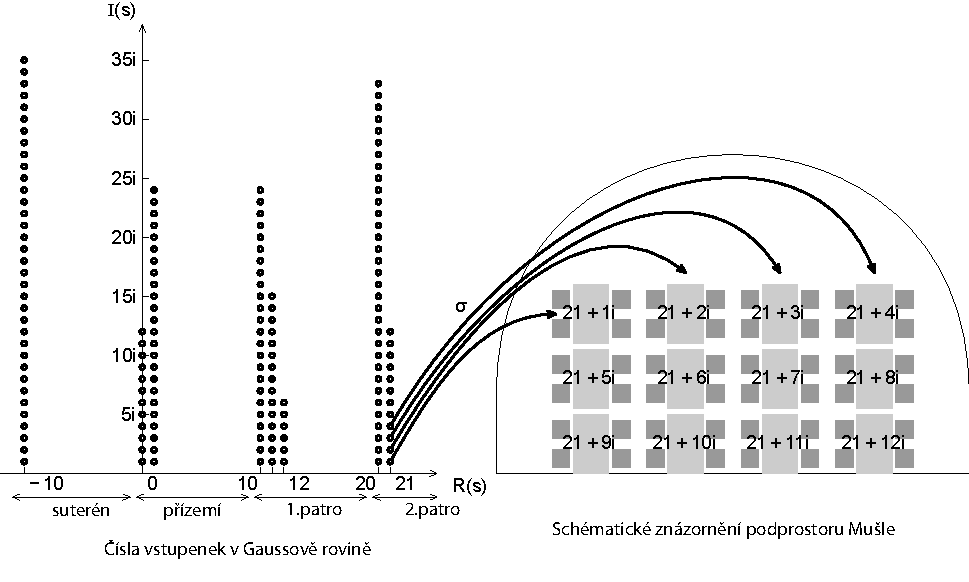
\includegraphics[scale=0.95]{bijekce.pdf}
\captionof{figure}{Bijekce $\sigma$ pro několik hodnot $s$}
\end{center}

\textbf{Věta 3} (Euler). Pro každé $x \in R$ a $y \in R$ platí
$$
e^{x+iy} = e^x (\cos y + i \sin y) 
$$
\par
\textit{Důkaz.}
Důkaz je na deštivý víkend, resp. na dva semestry.


\textbf{Definice 6}
(Značení stolů).
Na každém stolu $\Sigma \in \mathfrak{S}$ je v souladu s větou 9 uvedeno
číslo stolu s v přesném tvaru $s = \Re(s) + \Im(s) i$, které je vidět jen z určitého směru a dokud
jej někdo neodstraní. Z jiné strany stolu může být uvedeno číslo stolu navíc v alternativním
zápisu téhož komplexního čísla $s$ s možnou zaokrouhlovaí chybou.


\textbf{Věta 4}
(Hledání stolu).
Nechť $\Im(s) > 0$. Potom se matfyzák transportuje do správného
patra p Žofínského paláe podle lemmatu 7 a do příslušného podprostoru $\Pi$ s použitím
definie 4, kde podle definie 11 bude hledat stůl číslo $s$. (U stolu si zvolí židli podle
vlastního přání.)
\par
\textit{Důkaz.}
Důkaz je za "plesové" cvičení.


\textbf{Věta 5}
(O zoufalém tanečníkovi).
Zoufalý tanečník nemohouí najít svůj stůl použije
větu 10 či znovu si přečte definici 11 a prozkoumá značení stolů z jiného pohledu.
\par
\textit{Důkaz.}
Důkaz je zřejmý.


\textbf{Věta 6} (O zoufalém filosofovi). Nehť filosof zná číslo $s \in \check{\mathcal{Z}}^r_{\mathds{C}}$,
příp. má vstupenku $\lambda \in \Lambda_r$ s tímto číslem. Nechť na matfyzákém plese (v časoprostoru $\check{\mathcal{Z}}$)
je alespoò jeden matfyzák. Potom zoufalý filosof zvládne nalézti stůl, jemuž přísluší číslo $s$.
\par
Nyní předvedeme konstruktivní důkaz věty. Hlavní trik spočívá v tom, že záležitost
elegantně převedeme na snadno řešitelný problém.
\par
\textit{Důkaz.}
Předpokládáme, že v žofínském časoprostoru $\check{\mathcal{Z}}$ je alespoò jeden matfyzák
(což je zřejmě splněno z předpokladu věty), a současně víme,
že počet návštěvníků v $\check{\mathcal{Z}}$ je konečný
(pokud to neplyne z definie, plyne to z požárníh předpisů). Proto zoufalý filosof najde
matfyzáka v konečném čase, bude-li hledat šikovným způsobem, tj. každého hosta se zeptá
nejvýše jednou. Následně matfyzáka poprosí o pomoc s hledáním svého stolu a ukáže mu
vstupenku, resp. sdělí požadované číslo stolu $s$. Když matfyzák zná číslo $s$, vyřeší problém
podle věty 12, popřípadě věty 13. Správné řešení sdělí zoufalému filosovovi (samozřejmě
tak, aby jej pochopil), popř. ho ke stolu s dovede (jsme přece na Žofíně, který je normovaný
podle definie 1 (c)!). Tak se zoufalý filosof celý šťastný dostane ke stolu $\sigma(s)$. Q.E.D.
\footnote{Quod Erat Demonstrandum - Což bylo dokázati}



\end{document}